\documentclass{article}
\usepackage[utf8]{inputenc}
\usepackage{fancyhdr}
\usepackage{polski}
\usepackage{mathtools}
\usepackage{ulem}
\usepackage[margin = 1cm]{geometry}
\usepackage{hhline}
\usepackage{array}
\usepackage{booktabs}
\usepackage{tabularx}
\usepackage{colortbl}
\usepackage{longtable}
\usepackage{mathdots}
\usepackage{multirow}
\usepackage{centernot}
\usepackage{tensor}
\usepackage{fancyhdr}
\usepackage{lastpage}
\usepackage{enumitem}
\usepackage{amsthm}
\usepackage{mathabx}
\usepackage{algpseudocode}
\usepackage{algorithm}
\usepackage{graphicx}

\title{Systemy wbudowane '23 \\ Projekt \\ Automatyczne stacje meteorologiczne}
\author{Piotr Zapała, Igor Urbanowicz, Kacper Zawojski}
\date{March 2023}
\begin{document}
\maketitle
\begin{center}
    \large Automatyczna stacja meteorologiczna to system wbudowany, który służy do pomiaru i analizy danych meteorologicznych takich jak temperatura, wilgotność, ciśnienie atmosferyczne, prędkość wiatru, opady deszczu lub śniegu, a także promieniowanie słoneczne.
    \\[0.5cm]
    Automatyczny system pomiary i otrzymywanie wyników w formie cyfrowej pozwalają na 
    natychmiastową publikację oraz udostępnianie, co jest kluczową kwestią przy 
    prognozowaniu pogody oraz minimalizacji skutków klęsk żywiołowych, takich jak tornada, czy powodzie.
    Dzięki wykorzystaniu sieci Internet pomiary mogą być dostępne dla uytkowników znajdujących się drugim
    końcu globu. Ich cyfrowa postać pozwala na dowolne przetwarzanie, oprócz pomairu parametrów podstawowych
    można wyznaczyć wielkości dodatkowe, których uzyskiwanie jest czasochłonne lub niemożliwe przez obserwatora (np.temperatura wartości ekstremalnych) oraz wielkości pochodne (np. temperatura punktu rosy, temperatura odczuwalna).
    \\[0.5cm]
    Możliwa zaawansowana analiza statystyczna danych dostarcza znacznie więcej 
    dodatkowych informacji o pogodzie, pozwala pełniej wykorzystać wykonane pomiary. Stacje automatyczne 
    realizują złożone procedury oceny jakości danych, stanu technicznego aparatury, sygnalizują awarie, 
    dzięki temu zapewniając znacznie lepszą kontrolę jakości pomiarów. Automatyzacja pomiarów niesie za sobą 
    jednocześnie pewne dodatkowe wymagania. Stosowane w stacjach układy pomiarowe muszą mieć dodatkowe 
    parametry umożliwiające pracę bez nadzoru przez ustalony czas.
    \\[0.5cm]
    By wyniki były porównywalne niezbędna jest racjonalizacja i ujednolicenie algorytmów przetwarzania danych stąd wprowadzane procedury unifikacji dotyczące stosowanych przyrządów i procedur pomiarowych. Zbierane w celach synoptycznych dane muszą być 
    zgodne z wymaganiami WMO (World Meteorological Organization) oraz kompatybilne ze stacjami obsługowanymi.
    \\[0.5cm]
    \newpage
    Specyfikacja techniczna takiego układu może obejmować:
    \begin{flushleft}
        1. Układ czujników - to kluczowy element stacji meteorologicznej. Czujniki te są zaprojektowane w celu zbierania danych z otoczenia i przekazania ich do układu sterowania. Czujniki pomiarowe, które są najczęściej stosowane w stacjach meteorologicznych to: termometry, higrometry, barometry, anemometry i pluwiometry. Termometry służą do pomiaru temperatury, higrometry - do pomiaru wilgotności powietrza, barometry - do pomiaru ciśnienia atmosferycznego, anemometry - do pomiaru 
        prędkości i kierunku wiatru, a pluwiometry - do pomiaru opadów deszczu lub śniegu.
        \\[0.5cm]
        2. Komunikacja - jest to element, który umożliwia przesyłanie danych pomiarowych do innego systemu. Stacje meteorologiczne są zazwyczaj wyposażone w moduły komunikacyjne, takie jak Wi-Fi, Bluetooth lub RS-232. Wi-Fi i Bluetooth umożliwiają bezprzewodową komunikację, a RS-232 umożliwia komunikację za pomocą przewodów. Dzięki modułowi komunikacyjnemu, dane z czujników mogą być przesyłane na serwer lub na komputer, gdzie można je analizować i interpretować.
        3. Przetwarzanie danych - to element, który odpowiada za przetwarzanie danych pomiarowych zebranych przez czujniki. Układ przetwarzania danych jest najczęściej realizowany przez mikroprocesor lub mikrokontroler. Procesor może być programowany w języku C lub C++. W skład tego elementu mogą wchodzić też specjalne algorytmy, które przetwarzają dane z czujników i generują wyniki w postaci liczb lub grafów.
        \\[0.5cm]
        4. Interfejs użytkownika - jest to element, który umożliwia użytkownikom wgląd w dane pomiarowe. Interfejs użytkownika może przybierać różne formy, w zależności od rodzaju stacji meteorologicznej. Najczęściej stosowanymi interfejsami są wyświetlacze LCD lub interfejsy graficzne użytkownika (GUI). Wyświetlacze LCD są łatwe w obsłudze i zapewniają podstawowe informacje o warunkach pogodowych, takie jak temperatura, wilgotność i ciśnienie atmosferyczne. Interfejsy graficzne użytkownika są bardziej zaawansowane i pozwalają użytkownikom na wykonywanie różnych operacji, takich jak konfiguracja urządzenia lub generowanie raportów.
        \\[0.5cm]
        5. Zasilanie - jest to element, który umożliwia stacji meteorologicznej pracę w różnych warunkach terenowych. Stacje meteorologiczne są zazwyczaj zasilane przez baterię lub akumulator.
    \end{flushleft}
    
    \newpage

    \begin{center}
        \begin{tabular}{|l|l|l|}
        \hline
        \textbf{Nazwa PU:} Monitorowanie parametrów meteorologicznych & \textbf{Numer PU:} 1 & \textbf{Priorytet:} Wysoki \\
        \hline
        \hline
        \multicolumn{3}{|p{\dimexpr\linewidth-2\tabcolsep-2\arrayrulewidth}|}{\textbf{Aktor podstawowy:} Agencja meteorologiczna, Instytucja naukowa, Organizacja rządowa} \\
        \hline
        \hline
        \multicolumn{3}{|p{\dimexpr\linewidth-2\tabcolsep-2\arrayrulewidth}|}{\textbf{Typ opisu:} Szczegółowy} \\
        \hline
        \hline
        \multicolumn{3}{|p{\dimexpr\linewidth-2\tabcolsep-2\arrayrulewidth}|}{\textbf{Udziałowcy i cele:}
        \newline
        \textbf{Agencja meteorologiczna:}
        \newline
        Jeśli agencja meteorologiczna jest aktorem podstawowym, 
        to jej celem może być gromadzenie danych meteorologicznych w celu opracowania prognoz pogody
        oraz przewidywania i monitorowania zjawisk atmosferycznych takich jak huragany, tornada, trąby powietrzne,
        intensywne opady deszczu, itp.
        \newline 
        \textbf{Instytucja naukowa:}
        \newline
        Instytucje naukowe mogą być zainteresowane w badaniu i analizie danych meteorologicznych 
        dla celów badawczych, takich jak zrozumienie zmian klimatu i wpływu na środowisko naturalne.
        \newline
        \textbf{Organizacja rządowa:}
        \newline
        Organizacje rządowe, takie jak Ministerstwo Obrony Narodowej czy Straż Pożarna, mogą korzystać z
        danych meteorologicznych do podejmowania decyzji w zakresie zarządzania kryzysowym, np. w przypadku zagrożenia powodziowego
        czy innych zjawisk ekstremalnych. } \\
        \hline
        \hline
        \multicolumn{3}{|p{\dimexpr\linewidth-2\tabcolsep-2\arrayrulewidth}|}{\textbf{Wyzwalacz:} 
        W przypadku monitorowania parametrów meteorologicznych, wyzwalaczem może być np. zmiana
        warunków atmosferycznych lub potrzeba uzyskania aktualnych informacji o stanie pogody w danym obszarze.} \\
        \hline
        \hline
        \multicolumn{3}{|p{\dimexpr\linewidth-2\tabcolsep-2\arrayrulewidth}|}{\textbf{Typ wyzwalacza:}
        \newline
        \textbf{Wewnętrzne:}
        \newline
        -Przekroczenie określonej wartości przez jeden z monitorowanych parametrów (np. prędkości wiatru, opadów deszczu)
        \newline
        -Ustalony interwał czasowy, po którego upływie system automatycznie rozpoczyna monitorowanie parametrów meteorologicznych.
        \newline
        \textbf{Zewnętrzne:}
        \newline
        -Wskazanie przez użytkownika, że chce rozpocząć monitorowanie parametrów meteorologicznych
        \newline
        -Sygnał zewnętrzny z czujników meteorologicznych, który wskazuje na wystąpienie określonych warunków pogodowych} \\
        \hline
        \hline
        \multicolumn{3}{|p{\dimexpr\linewidth-2\tabcolsep-2\arrayrulewidth}|}{\textbf{Asocjacja:}
        z PU dotyczącym przewidywania warunków pogodowych, ponieważ monitorowanie parametrów
        meteorologicznych może dostarczać danych wejściowych dla algorytmów przewidywania pogody.} \\
        \hline
        \hline
        \multicolumn{3}{|p{\dimexpr\linewidth-2\tabcolsep-2\arrayrulewidth}|}{\textbf{Zawieranie:}
        \newline
        -Zbieranie i przetwarzanie danych z czujników meteorologicznych
        \newline
        -Analiza i generowanie prognoz pogody na podstawie zebranych danych
        \newline
        -Alarmowanie w przypadku niebezpiecznych warunków pogodowych
        \newline
        -Wykonywanie testów jakości danych meteorologicznych} \\
        \hline
        \hline
        \multicolumn{3}{|p{\dimexpr\linewidth-2\tabcolsep-2\arrayrulewidth}|}{\textbf{Rozszerzenie:}
        \newline
        \textbf{PU "Zapis danych meteorologicznych do bazy danych":} dodanie przepływu umożliwiającego zapisywanie danych meteorologicznych do bazy danych w trakcie monitorowania parametrów meteorologicznych.
        \newline
        \textbf{PU "Zarządzanie alertami meteorologicznymi":} w przypadku wykrycia ekstremalnych warunków pogodowych, PU "Monitorowanie parametrów meteorologicznych" może uruchamiać PU "Zarządzanie alertami meteorologicznymi",
        który ma na celu przekazanie ostrzeżeń i zaleceń dotyczących bezpieczeństwa publicznego, takich jak ewakuacja lub szukanie schronienia.
        \newline
        \textbf{PU "Prognozowanie pogody":} dane meteorologiczne mogą być wykorzystywane przez PU "Prognozowanie pogody", aby opracować prognozy na kilka dni do przodu.} \\
        \hline
        \hline
        \multicolumn{3}{|p{\dimexpr\linewidth-2\tabcolsep-2\arrayrulewidth}|}{\textbf{Generalizacja:}
        z PU dotyczącym monitorowania różnych parametrów środowiskowych, ponieważ system monitorowania
        może obejmować nie tylko parametry meteorologiczne, ale także inne parametry, takie jak jakość powietrza czy hałas.} \\
        \hline
        \end{tabular}
    \end{center}

    \newpage

    \begin{center}
        \begin{tabular}{|l|l|l|}
        \hline
        \multicolumn{3}{|p{\dimexpr\linewidth-2\tabcolsep-2\arrayrulewidth}|}{\textbf{Zwykły przepływ zdarzeń:}
        \newline
        \textbf{1.} Wyzwalacz wewnętrzny (np. timeout) lub zewnętrzny (np. naciśnięcie przycisku "start") uruchamia PU.
        \newline
        \textbf{2.} PU rozpoczyna monitorowanie parametrów meteorologicznych (temperatura, wilgotność, ciśnienie atmosferyczne itp.) z użyciem odpowiednich czujników i urządzeń.
        \newline
        \textbf{3.} Dane odczytywane przez czujniki są przetwarzane i zapisywane w pamięci wewnętrznej lub na zewnętrznych nośnikach danych.
        \newline
        \textbf{4.} PU regularnie przesyła dane do systemu nadzorczego lub do innych urządzeń, takich jak systemy alarmowe.
        \newline
        \textbf{5.} W przypadku wykrycia anomalii lub przekroczenia ustalonych progów alarmowych, PU generuje alert i/lub aktywuje odpowiednie urządzenia do podjęcia innych działań.
        \newline
        \textbf{6.} Po zakończeniu monitorowania, PU zostaje wyłączony lub przechodzi w tryb uśpienia, oczekując na kolejny wyzwalacz.} \\
        \hline
        \hline
        \multicolumn{3}{|p{\dimexpr\linewidth-2\tabcolsep-2\arrayrulewidth}|}{\textbf{Przepływy poboczne:}
        \newline 
        \textbf{1.} Przypadek, gdy brakujące dane meteorologiczne są uzupełniane na podstawie modeli matematycznych lub historycznych danych.
        \newline
        \textbf{2.} Przypadek, gdy poziom niektórych parametrów przekracza określone progi alarmowe, co wymaga powiadomienia odpowiednich służb lub włączenia specjalnych procedur.} \\
        \hline
        \hline
        \multicolumn{3}{|p{\dimexpr\linewidth-2\tabcolsep-2\arrayrulewidth}|}{\textbf{Przepływy alternatywne/wyjątkowe:}
        \newline
        \textbf{1.} Brak połączenia z urządzeniem pomiarowym - w takim przypadku system powinien zareagować w sposób odpowiedni i poinformować użytkownika o problemie.
        \newline
        \textbf{2.} Awaria czujnika - jeśli w trakcie monitorowania parametrów atmosferycznych czujnik ulegnie awarii, system powinien wyświetlić odpowiednie ostrzeżenie lub powiadomienie, aby użytkownik mógł podjąć odpowiednie kroki w celu naprawy lub wymiany czujnika.
        \newline
        \textbf{3.} Nieprawidłowe odczyty parametrów - w niektórych przypadkach parametry atmosferyczne mogą zostać źle odczytane lub zinterpretowane przez system. W takim przypadku system powinien wyświetlić odpowiednie ostrzeżenie lub powiadomienie, aby użytkownik mógł skorygować odczyty.
        \newline
        \textbf{4.} Problem z zasilaniem - w przypadku utraty zasilania system powinien zareagować w sposób odpowiedni i poinformować użytkownika o problemie, a także podjąć kroki w celu zachowania ostatnich pomiarów przed wyłączeniem urządzenia.
        \newline
        \textbf{5.} Zmiana ustawień pomiarowych - użytkownik może chcieć zmienić ustawienia pomiarowe w zależności od sytuacji. System powinien umożliwić zmianę tych ustawień i odpowiednio reagować na zmiany.} \\
        \hline
        \end{tabular}
    \end{center}    

    \newpage

    \begin{center}
        \begin{tabular}{|l|l|l|}
        \hline
        \textbf{Nazwa PU:} Generowanie raportów pogodowych & \textbf{Numer PU:} 2 & \textbf{Priorytet:} Wysoki \\
        \hline
        \hline
        \multicolumn{3}{|p{\dimexpr\linewidth-2\tabcolsep-2\arrayrulewidth}|}{\textbf{Aktor podstawowy:}
        \newline 
        Aktor podstawowy dla Generowania raportów pogodowych to z reguły system lub aplikacja,
        która na podstawie zebranych parametrów meteorologicznych generuje odpowiednie raporty.
        Może to być na przykład system monitorujący warunki atmosferyczne na lotnisku,
        który automatycznie generuje raporty dla personelu obsługującego starty i lądowania samolotów.} \\
        \hline
        \hline
        \multicolumn{3}{|p{\dimexpr\linewidth-2\tabcolsep-2\arrayrulewidth}|}{\textbf{Typ opisu:} Szczegółowy} \\
        \hline
        \hline
        \multicolumn{3}{|p{\dimexpr\linewidth-2\tabcolsep-2\arrayrulewidth}|}{\textbf{Udziałowcy i cele:}
        \newline
        \textbf{Pracownicy służb meteorologicznych} odpowiedzialni za zbieranie i przetwarzanie danych meteorologicznych.
        \newline
        \textbf{Programiści i analitycy danych} odpowiedzialni za opracowanie narzędzi do generowania raportów.
        \newline
        \textbf{Pracownicy administracyjni} odpowiedzialni za dystrybucję i udostępnianie raportów.} \\
        \hline
        \hline
        \multicolumn{3}{|p{\dimexpr\linewidth-2\tabcolsep-2\arrayrulewidth}|}{\textbf{Wyzwalacz:}
        Wyzwalaczem dla Generowania raportów pogodowych może być żądanie użytkownika systemu,
        określona data i godzina, lub inny program lub system, który potrzebuje aktualnych raportów pogodowych.} \\
        \hline
        \hline
        \multicolumn{3}{|p{\dimexpr\linewidth-2\tabcolsep-2\arrayrulewidth}|}{\textbf{Typ wyzwalacza:}
        \newline
        \textbf{Wewnętrzne:}
        \newline
        -Ustawienie określonego czasu (np. co 24 godziny), w którym system automatycznie generuje raport pogodowy.
        \newline
        \textbf{Zewnętrzne:}
        \newline
        -Zlecenie generowania raportu przez użytkownika poprzez interfejs użytkownika.
        \newline
        -Sensor meteorologiczny, który informuje system o określonych warunkach pogodowych, co skutkuje automatycznym wygenerowaniem raportu.} \\
        \hline
        \hline
        \multicolumn{3}{|p{\dimexpr\linewidth-2\tabcolsep-2\arrayrulewidth}|}{\textbf{Asocjacja:}
        \newline
        Generowanie raportów pogodowych może być powiązane z innymi PU, takimi jak:
        \newline
        -Monitorowanie parametrów meteorologicznych
        \newline
        -Analiza danych meteorologicznych
        \newline
        -Przechowywanie danych meteorologicznych
        \newline
        -Udostępnianie danych meteorologicznych użytkownikom
        \newline
        -Wizualizacja danych meteorologicznych} \\
        \hline
        \hline
        \multicolumn{3}{|p{\dimexpr\linewidth-2\tabcolsep-2\arrayrulewidth}|}{\textbf{Zawieranie:}
        \newline
        \textbf{1.} Przetwarzanie danych meteorologicznych i generowanie prognozy pogody na podstawie modeli numerycznych.
        \newline
        \textbf{2.} Analizowanie danych i generowanie raportów z informacjami o temperaturze, opadach, wietrze, wilgotności, ciśnieniu itp.
        \newline
        \textbf{3.} Udostępnianie raportów w różnych formatach (np. tekstowy, graficzny) i kanałach (np. strona internetowa, aplikacja mobilna, media społecznościowe).
        \newline
        \textbf{4.} Archiwizowanie danych meteorologicznych i raportów pogodowych.
        \newline
        \textbf{5.} Monitorowanie jakości danych i dokonywanie korekt w przypadku wykrycia błędów.} \\
        \hline
        \hline
        \multicolumn{3}{|p{\dimexpr\linewidth-2\tabcolsep-2\arrayrulewidth}|}{\textbf{Rozszerzenie:}
        \newline
        \textbf{1.} Rozszerzenie o automatyczne generowanie raportów na podstawie określonych kryteriów, takich jak poziom opadów, temperatura, wilgotność itp. W tym przypadku można rozważyć zintegrowanie z innymi systemami, takimi jak czujniki pogodowe, aby automatycznie pobierać dane i generować raporty.
        \newline
        \textbf{2.} Rozszerzenie o możliwość generowania map pogodowych, które pokazują zmiany pogodowe na danym obszarze. W tym przypadku może być potrzebna integracja z systemami GIS oraz danymi satelitarnymi.
        \newline
        \textbf{3.} Rozszerzenie o integrację z systemami alarmowymi, które wyświetlają alerty meteorologiczne w przypadku, gdy poziom opadów, prędkość wiatru lub inne parametry przekraczają określony próg.
        \newline
        \textbf{4.} Rozszerzenie o możliwość generowania prognoz pogodowych na podstawie danych historycznych i modeli matematycznych. W tym przypadku konieczna jest integracja z systemami modelowania numerycznego i algorytmami przewidywania pogody.} \\
        \hline
        \end{tabular}
    \end{center}

    \begin{center}
        \begin{tabular}{|l|l|l|}
        \hline
        \multicolumn{3}{|p{\dimexpr\linewidth-2\tabcolsep-2\arrayrulewidth}|}{\textbf{Generalizacja:}
        \newline
        \textbf{1.} System monitorowania parametrów atmosferycznych - jako narzędzie zbierające dane meteorologiczne, które będą używane do generowania raportów pogodowych.
        \newline
        \textbf{2.} System generowania raportów - jako podsystem generujący raporty pogodowe na podstawie danych meteorologicznych.
        \newline
        \textbf{3.} Interfejs użytkownika - jako interfejs pozwalający użytkownikom na wybór parametrów, na podstawie których będą generowane raporty pogodowe.
        \newline
        \textbf{4.} System powiadomień - jako system powiadamiający użytkowników o nowych raportach pogodowych i innych istotnych informacjach.
        \newline
        \textbf{5.} System bazy danych - jako narzędzie przechowujące dane meteorologiczne i informacje o wygenerowanych raportach pogodowych.} \\
        \hline
        \hline
        \multicolumn{3}{|p{\dimexpr\linewidth-2\tabcolsep-2\arrayrulewidth}|}{\textbf{Zwykły przepływ zdarzeń:}
        \newline
        Przykładowy zwykły przepływ zdarzeń dla przypadku użycia "Generowanie raportów pogodowych" może wyglądać następująco:
        \newline
        \textbf{1.} System odczytuje aktualne dane z czujników atmosferycznych.
        \newline
        \textbf{2.} System porównuje odczytane dane z prognozą pogody dla danej lokalizacji.
        \newline
        \textbf{3.} System generuje raport pogodowy na podstawie odczytów z czujników oraz prognozy pogody.
        \newline
        \textbf{4.} Raport jest zapisywany w wyznaczonym miejscu.
        \newline
        \textbf{5.} System wyświetla informację o poprawnym wykonaniu operacji.} \\
        \hline
        \hline
        \multicolumn{3}{|p{\dimexpr\linewidth-2\tabcolsep-2\arrayrulewidth}|}{\textbf{Przepływy poboczne:}
        \newline
        \textbf{1.} Zgłoszenie awarii lub błędu w działaniu stacji, co może wymagać interwencji technicznej lub naprawy.
        \newline
        \textbf{2.} W przypadku nagłych zmian warunków atmosferycznych, takich jak silne wiatry, ulewy lub burze, możliwe jest, że stacja będzie potrzebować dodatkowych czynności w celu monitorowania i raportowania tych zdarzeń.
        \newline
        \textbf{3.} Konieczność przeprowadzenia regularnych przeglądów i konserwacji stacji w celu utrzymania jej w pełnej sprawności i zapewnienia dokładności raportów.
        \newline
        \textbf{4.} Konieczność aktualizacji oprogramowania stacji, aby uwzględnić nowe technologie i ulepszenia w zakresie monitorowania warunków atmosferycznych.
        \newline
        \textbf{5.} W przypadku wykrycia błędów lub niedoskonałości w raportach, może zajść konieczność przeprowadzenia dodatkowych badań lub analiz w celu poprawy dokładności raportów.} \\
        \hline
        \hline
        \multicolumn{3}{|p{\dimexpr\linewidth-2\tabcolsep-2\arrayrulewidth}|}{\textbf{Przepływy alternatywne/wyjątkowe:}
        \newline
        \textbf{1.} Awaryjne zasilanie stacji meteorologicznej w przypadku przerwy w dostawie energii elektrycznej.
        \newline
        \textbf{2.} Przerwanie generowania raportów w przypadku braku połączenia z internetem lub awarii systemu przetwarzania danych.
        \newline
        \textbf{3.} Awaria automatycznej stacji meteorologicznej, co może wymagać manualnego pomiaru i wprowadzenia danych do systemu generującego raporty.
        \newline
        \textbf{4.} Utrata połączenia z siecią internetową, co może uniemożliwić przesłanie raportów na serwer.
        \newline
        \textbf{5.} Błędy w odczycie danych z automatycznej stacji meteorologicznej, co może wymagać ręcznego wprowadzenia poprawek lub podjęcia innych działań korygujących.
        \newline
        \textbf{6.} Brak dostępności niektórych danych meteorologicznych, co może skutkować brakiem pewnych informacji w raportach lub koniecznością wykorzystania innych źródeł danych.} \\
        \hline
        \end{tabular}
    \end{center}

    \newpage

    \begin{center}
        \begin{tabular}{|l|l|l|}
        \hline
        & & \\[-2ex]
        \textbf{Nazwa PU:} Alarmowanie w przypadku niebezpiecznych \\ warunków pogodowych & \textbf{Numer PU:} 3 & \textbf{Priorytet:} Wysoki \\ & & \\
        \hline
        \hline
        \multicolumn{3}{|p{\dimexpr\linewidth-2\tabcolsep-2\arrayrulewidth}|}{\textbf{Aktor podstawowy:}
        \newline
        Głównym wykonawcą/interesantem przypadku użycia "Alarmowanie w przypadku niebezpiecznych warunków pogodowych"
        może być np. administracja publiczna (np. władze miasta lub gminy), służby ratownicze (np. straż pożarna, pogotowie ratunkowe),
        firmy transportowe lub linie lotnicze, które muszą dostosować swoje działania do aktualnych warunków pogodowych,
        a także zwykli użytkownicy, którzy chcą być informowani o niebezpiecznych sytuacjach i podjąć odpowiednie środki ostrożności.} \\
        \hline
        \hline
        \multicolumn{3}{|p{\dimexpr\linewidth-2\tabcolsep-2\arrayrulewidth}|}{\textbf{Typ opisu:} Szczegółowy} \\
        \hline
        \hline
        \multicolumn{3}{|p{\dimexpr\linewidth-2\tabcolsep-2\arrayrulewidth}|}{\textbf{Udziałowcy i cele:}
        \newline
        \textbf{Udziałowcy:}
        \newline
        \textbf{Stacja meteorologiczna} - dostarcza informacji o parametrach atmosferycznych.
        \newline
        \textbf{System alarmowy} - służy do wykrywania niebezpiecznych warunków pogodowych i przekazywania informacji o nich.
        \newline
        \textbf{Operator stacji meteorologicznej} - odpowiada za monitorowanie parametrów atmosferycznych oraz reagowanie na wykryte niebezpieczne warunki.
        \newline
        \textbf{Użytkownicy} - otrzymują informacje o niebezpiecznych warunkach pogodowych i podejmują odpowiednie działania mające na celu zapewnienie swojego bezpieczeństwa.
        \newline
        \textbf{Cele udziałowców:}
        \newline
        \textbf{Stacja meteorologiczna} - dostarczenie dokładnych informacji o parametrach atmosferycznych.
        \newline
        \textbf{System alarmowy} - wykrycie niebezpiecznych warunków pogodowych i przekazanie informacji o nich operatorowi stacji meteorologicznej.
        \newline
        \textbf{Operator stacji meteorologicznej} - szybka reakcja na wykryte niebezpieczne warunki pogodowe poprzez wydanie alarmu.
        \newline
        \textbf{Użytkownicy} - otrzymanie ostrzeżenia o niebezpiecznych warunkach pogodowych i podjęcie odpowiednich działań mających na celu zminimalizowanie ryzyka dla siebie i swojego otoczenia.} \\
        \hline
        \hline
        \multicolumn{3}{|p{\dimexpr\linewidth-2\tabcolsep-2\arrayrulewidth}|}{\textbf{Wyzwalacz:}
        \newline 
        W przypadku użycia "Alarmowanie w przypadku niebezpiecznych warunków pogodowych",
        wyzwalaczem może być wykrycie niebezpiecznych warunków pogodowych przez stację meteorologiczną
        lub inny system monitorowania, który może przesłać sygnał do systemu alarmowego. 
        Sygnał ten może być również manualnie inicjowany przez operatora systemu w przypadku
        uzyskania informacji o niebezpiecznych warunkach pogodowych.} \\
        \hline
        \hline
        \multicolumn{3}{|p{\dimexpr\linewidth-2\tabcolsep-2\arrayrulewidth}|}{\textbf{Typ wyzwalacza:}
        \newline
        \textbf{Zewnętrzny:}
        \newline
        -Detekcja przez stację meteorologiczną warunków pogodowych takich jak silny wiatr,
        ulewny deszcz, burze, itp. i wysłanie powiadomienia lub alarmu do odpowiednich służb lub osób.} \\
        \hline
        \hline
        \multicolumn{3}{|p{\dimexpr\linewidth-2\tabcolsep-2\arrayrulewidth}|}{\textbf{Asocjacja:}
        \newline
        Przypadek użycia "Alarmowanie w przypadku niebezpiecznych warunków pogodowych"
        może być powiązany z innymi przypadkami użycia związanymi z generowaniem i przetwarzaniem
        danych meteorologicznych, np. "Generowanie raportów pogodowych" lub "Monitorowanie warunków atmosferycznych".} \\
        \hline
        \hline
        \multicolumn{3}{|p{\dimexpr\linewidth-2\tabcolsep-2\arrayrulewidth}|}{\textbf{Zawieranie:}
        \newline
        \textbf{1.} Generowanie raportów pogodowych - aby uzyskać aktualne informacje o warunkach pogodowych.
        \newline
        \textbf{2.} Analiza warunków pogodowych - aby ocenić, czy warunki są niebezpieczne i wymagają alarmowania.
        \newline
        \textbf{3.} Wysyłanie powiadomień - aby poinformować odpowiednie osoby o niebezpiecznych warunkach pogodowych.
        \newline
        \textbf{4.} Zarządzanie listami odbiorców powiadomień - aby umożliwić użytkownikom dodawanie, usuwanie i modyfikowanie list odbiorców powiadomień.
        \newline
        \textbf{5.} Konfiguracja alarmów - aby umożliwić użytkownikom ustawienie parametrów alarmów, takich jak poziom zagrożenia pogodowego i rodzaj powiadomień.} \\
        \hline
        \end{tabular}
    \end{center}

    \begin{center}
        \begin{tabular}{|l|l|l|}
        \hline
        \multicolumn{3}{|p{\dimexpr\linewidth-2\tabcolsep-2\arrayrulewidth}|}{\textbf{Rozszerzenie:}
        \newline
        Automatyczne wyłączenie systemów zasilania awaryjnego w przypadku, gdy pogoda wraca do normalnego stanu
        i nie ma już zagrożenia dla systemów. Może to wymagać dodatkowych przepływów,
        takich jak monitorowanie stanu systemów, wykrywanie zmian w warunkach pogodowych
        i podejmowanie decyzji o wyłączeniu systemów na podstawie tych informacji.} \\
        \hline
        \hline
        \multicolumn{3}{|p{\dimexpr\linewidth-2\tabcolsep-2\arrayrulewidth}|}{\textbf{Generalizacja:} -----------------||----------------- } \\
        \hline
        \hline
        \multicolumn{3}{|p{\dimexpr\linewidth-2\tabcolsep-2\arrayrulewidth}|}{\textbf{Zwykły przepływ zdarzeń:}
        \newline
        \textbf{1.} Automatyczna stacja meteorologiczna monitoruje warunki pogodowe w danym regionie.
        \newline
        \textbf{2.} Jeśli warunki pogodowe spełniają kryteria uznane za niebezpieczne, stacja generuje alarm.
        \newline
        \textbf{3.} Alarm zostaje przesłany do systemu alarmowego.
        \newline
        \textbf{4.} System alarmowy podejmuje decyzję o dalszych działaniach w zależności od rodzaju alarmu i jego priorytetu.
        \newline
        \textbf{5.} W przypadku alarmu o wysokim priorytecie, system alarmowy natychmiast powiadamia odpowiednie służby ratownicze, takie jak straż pożarna, policja czy pogotowie ratunkowe.
        \newline
        \textbf{6.} Służby ratownicze podejmują dalsze kroki w celu przeciwdziałania skutkom niebezpiecznych warunków pogodowych, takie jak ewakuacja ludzi z zagrożonych obszarów czy interwencja w przypadku katastrof naturalnych.} \\
        \hline
        \hline
        \multicolumn{3}{|p{\dimexpr\linewidth-2\tabcolsep-2\arrayrulewidth}|}{\textbf{Przepływy poboczne:}
        \newline
        \textbf{1.} Utrata połączenia z urządzeniem meteorologicznym podczas pobierania informacji o warunkach pogodowych.
        \newline
        \textbf{2.} Zmiana progów alarmowania w zależności od konkretnych wymagań użytkownika.
        \newline
        \textbf{3.} Ograniczenie liczby powiadomień w ciągu określonego czasu, aby uniknąć natłoku informacji.
        \newline
        \textbf{4.} Wyłączenie alarmów na życzenie użytkownika, na przykład w przypadku fałszywego alarmu lub wyłączenia funkcji alarmowej w ogóle.} \\
        \hline
        \hline
        \multicolumn{3}{|p{\dimexpr\linewidth-2\tabcolsep-2\arrayrulewidth}|}{\textbf{Przepływy alternatywne/wyjątkowe:}
        \newline
        \textbf{1.} Awaria stacji meteorologicznej - jeśli stacja meteorologiczna przestanie działać, może być konieczne użycie alternatywnych źródeł informacji o warunkach pogodowych, takich jak inne stacje meteorologiczne lub systemy satelitarne.
        \newline
        \textbf{2.} Brak zasięgu lub awaria sieci internetowej - jeśli system alarmowania jest zintegrowany z internetem, może wystąpić problem z połączeniem, co uniemożliwi wysłanie powiadomień o niebezpiecznych warunkach pogodowych. W takim przypadku można skorzystać z alternatywnych sposobów komunikacji, takich jak SMS lub sygnały dźwiękowe.
        \newline
        \textbf{3.} Wysoka liczba zgłoszeń - w przypadku bardzo wysokiej liczby zgłoszeń o niebezpiecznych warunkach pogodowych, system alarmowy może nie być w stanie przetworzyć wszystkich powiadomień. W takim przypadku konieczne może być zastosowanie priorytetów i selekcji powiadomień w oparciu o kryteria takie jak lokalizacja czy zagrożenie.
        \newline
        \textbf{4.} Brak reakcji użytkowników - w przypadku gdy użytkownicy ignorują powiadomienia o niebezpiecznych warunkach pogodowych, konieczne może być zastosowanie alternatywnych sposobów informowania, takich jak komunikaty dźwiękowe czy powiadomienia tekstowe.} \\
        \hline
        \end{tabular}
    \end{center}

    \newpage

    \begin{center}
        \begin{tabular}{|l|l|l|}
        \hline
        \textbf{Nazwa PU:} Konfiguracja automatycznej stacji meteorologicznej & \textbf{Numer PU:} 4 & \textbf{Priorytet:} Wysoki \\
        \hline
        \hline
        \multicolumn{3}{|p{\dimexpr\linewidth-2\tabcolsep-2\arrayrulewidth}|}{\textbf{Aktor podstawowy:}
        \newline 
        Aktor podstawowy w przypadku konfiguracji automatycznej stacji meteorologicznej to zwykle osoba
        lub zespół odpowiedzialny za instalację, uruchomienie i konfigurację stacji meteorologicznej.
        Może to być na przykład inżynier meteorologii, technik serwisowy lub inna osoba związana z działem
        meteorologicznym lub naukowym. Oprócz tego, osoby odpowiedzialne za przetwarzanie i wykorzystanie
        danych ze stacji meteorologicznej również mogą być zainteresowane konfiguracją stacji,
        aby zapewnić odpowiednie parametry i jakość pomiarów.} \\
        \hline
        \hline
        \multicolumn{3}{|p{\dimexpr\linewidth-2\tabcolsep-2\arrayrulewidth}|}{\textbf{Typ opisu:} Szczegółowy} \\
        \hline
        \hline
        \multicolumn{3}{|p{\dimexpr\linewidth-2\tabcolsep-2\arrayrulewidth}|}{\textbf{Udziałowcy i cele:}
        \newline
        \textbf{Udziałowcy:} 
        \newline
        \textbf{Administrator systemu lub osoba odpowiedzialna za utrzymanie stacji meteorologicznej} - główny wykonawca, który będzie konfigurował urządzenie i dokonywał ustawień.
        \newline
        \textbf{Użytkownicy stacji meteorologicznej} - osoby, które będą korzystać z danych i informacji generowanych przez stację.
        \newline
        \textbf{Inne systemy lub urządzenia}, które będą odbierać dane z stacji meteorologicznej lub przetwarzać je w jakikolwiek sposób.
        \newline 
        \textbf{Cele udziałowców:}
        \newline
        \textbf{Administrator systemu} lub osoba odpowiedzialna za utrzymanie stacji meteorologicznej może mieć na celu dostosowanie stacji do konkretnych wymagań lub warunków, a także zapewnienie jej poprawnego funkcjonowania i bezpieczeństwa.
        \newline
        \textbf{Użytkownicy} stacji meteorologicznej mogą chcieć korzystać z danych i informacji generowanych przez stację w celach naukowych, badawczych lub komercyjnych.
        \newline
        \textbf{Inne systemy lub urządzenia}, które będą odbierać dane z stacji meteorologicznej lub przetwarzać je w jakikolwiek sposób, mogą mieć na celu integrację tych danych z innymi systemami lub urządzeniami w celu dokładniejszej analizy lub wizualizacji informacji meteorologicznych.} \\
        \hline
        \hline
        \multicolumn{3}{|p{\dimexpr\linewidth-2\tabcolsep-2\arrayrulewidth}|}{\textbf{Wyzwalacz:}
        \newline
        -Nowe urządzenie, które ma zostać dodane do stacji meteorologicznej
        \newline
        -Zmiana ustawień istniejącego urządzenia (np. zmiana częstotliwości pomiarów)
        \newline
        -Zlecenie serwisowe dotyczące stacji meteorologicznej
        \newline
        -Wykrycie problemów technicznych w stacji meteorologicznej.} \\
        \hline
        \hline
        \multicolumn{3}{|p{\dimexpr\linewidth-2\tabcolsep-2\arrayrulewidth}|}{\textbf{Typ wyzwalacza:}
        \newline
        \textbf{Wewnętrzne:}
        \newline 
        -Automatyczne uruchomienie procesu konfiguracji po pierwszym uruchomieniu stacji lub po zresetowaniu jej ustawień. 
        \newline
        \textbf{Zewnętrzny:}
        \newline
        -Ręczna inicjacja procesu konfiguracji przez operatora lub program automatyczny wywołujący tę czynność w odpowiedzi na określone warunki pogodowe lub potrzeby użytkownika.} \\
        \hline
        \hline
        \multicolumn{3}{|p{\dimexpr\linewidth-2\tabcolsep-2\arrayrulewidth}|}{\textbf{Asocjacja:}
        \newline
        Przypadek użycia "Konfiguracja Automatycznej stacji meteorologicznej" może być powiązany
        z innymi przypadkami użycia, takimi jak "Zbieranie danych z automatycznej stacji meteorologicznej",
        "Przechowywanie danych z automatycznej stacji meteorologicznej" lub "Analiza danych z automatycznej stacji meteorologicznej".
        Wszystkie te przypadki użycia są ze sobą powiązane poprzez wspólne wykorzystanie danych ze stacji meteorologicznej.} \\
        \hline
        \hline
        \multicolumn{3}{|p{\dimexpr\linewidth-2\tabcolsep-2\arrayrulewidth}|}{\textbf{Zawieranie:}
        \newline
        -Konfiguracja połączenia z siecią internetową
        \newline
        -Konfiguracja czujników meteorologicznych
        \newline
        -Przeprowadzenie testów diagnostycznych stacji
        \newline
        -Konfiguracja systemu zapisu danych
        \newline
        -Konfiguracja systemu alarmowego na niebezpieczne warunki pogodowe
        \newline
        -Konfiguracja protokołu komunikacyjnego z urządzeniami zewnętrznymi} \\
        \hline
        \end{tabular}
    \end{center}

    \newpage 

    \begin{center}
        \begin{tabular}{|l|l|l|}
        \hline
        \multicolumn{3}{|p{\dimexpr\linewidth-2\tabcolsep-2\arrayrulewidth}|}{\textbf{Rozszerzenie:} -----------------||-----------------} \\
        \hline
        \hline
        \multicolumn{3}{|p{\dimexpr\linewidth-2\tabcolsep-2\arrayrulewidth}|}{\textbf{Generalizacja:} -----------------||-----------------} \\
        \hline
        \hline
        \multicolumn{3}{|p{\dimexpr\linewidth-2\tabcolsep-2\arrayrulewidth}|}{\textbf{Zwykły przepływ zdarzeń:}
        \newline
        \textbf{1.} Uruchomienie programu konfiguracyjnego stacji meteorologicznej.
        \newline
        \textbf{2.} Wybór języka i regionu dla stacji.
        \newline
        \textbf{3.} Wybór rodzaju połączenia z serwerem internetowym.
        \newline
        \textbf{4.} Podanie nazwy użytkownika i hasła do konta na serwerze.
        \newline
        \textbf{5.} Wybór preferencji dotyczących formatu danych pomiarowych.
        \newline
        \textbf{6.} Wybór preferencji dotyczących częstotliwości aktualizacji danych.
        \newline
        \textbf{7.} Ustawienie stacji meteorologicznej w wyznaczonej lokalizacji.
        \newline
        \textbf{8.} Rozpoczęcie regularnego pobierania i wysyłania danych pomiarowych do serwera internetowego.
        \newline
        \textbf{9.} Monitorowanie jakości połączenia i reagowanie na ewentualne błędy lub problemy z połączeniem.
        \newline
        \textbf{10.} Zakończenie programu konfiguracyjnego lub przejście do trybu monitorowania danych.} \\
        \hline
        \hline
        \multicolumn{3}{|p{\dimexpr\linewidth-2\tabcolsep-2\arrayrulewidth}|}{\textbf{Przepływy poboczne:}
        \newline
        \textbf{1.} Niepowodzenie w komunikacji z urządzeniami pomiarowymi: w przypadku, gdy urządzenia pomiarowe nie odpowiadają na zapytania, aplikacja może próbować połączyć się ponownie lub wyświetlić stosowny komunikat o błędzie.
        \newline
        \textbf{2.} Ustawienie niewłaściwych parametrów pomiarowych: użytkownik może wprowadzić niewłaściwe parametry pomiarowe, takie jak interwał pomiaru, zakres pomiarów, itp. Aplikacja może wtedy wyświetlić stosowny komunikat ostrzegający użytkownika przed skutkami niewłaściwego ustawienia parametrów.
        \newline
        \textbf{3.} Niepowodzenie w przetwarzaniu danych: jeśli wystąpił problem z przetwarzaniem danych z urządzeń pomiarowych, aplikacja może wyświetlić komunikat o błędzie i poprosić użytkownika o podjęcie odpowiednich działań, np. sprawdzenie połączenia z urządzeniami pomiarowymi lub konfigurację aplikacji.
        \newline
        \textbf{4.} Konflikt z innymi aplikacjami: aplikacja może wykryć konflikt z innymi programami lub urządzeniami, które korzystają z tych samych zasobów, takich jak porty komunikacyjne lub kanały danych. W takim przypadku aplikacja może powiadomić użytkownika o konflikcie i poprosić o rozwiązanie problemu.
        \newline
        \textbf{5.} Niepowodzenie w zapisie danych: aplikacja może napotkać problemy z zapisem danych pomiarowych do bazy danych lub plików. W takim przypadku aplikacja może wyświetlić stosowny komunikat o błędzie i poprosić użytkownika o podjęcie odpowiednich działań, np. o sprawdzenie dysku lub dostępność miejsca na dysku.} \\
        \hline
        \hline
        \multicolumn{3}{|p{\dimexpr\linewidth-2\tabcolsep-2\arrayrulewidth}|}{\textbf{Przepływy alternatywne/wyjątkowe:}
        \newline
        \textbf{1.} Wyjątkowe warunki pogodowe: W przypadku wystąpienia wyjątkowych warunków pogodowych (takich jak burze, silne wiatry, opady śniegu), system automatycznie podejmuje decyzję o wykonaniu dodatkowych pomiarów i wysłaniu alarmu w przypadku wykrycia niebezpiecznych warunków pogodowych.
        \newline
        \textbf{2.} Zgłoszenie błędu: Jeśli zostanie zgłoszony błąd w działaniu stacji meteorologicznej, system podejmuje decyzję o przeprowadzeniu diagnostyki i naprawie, co może składać się z kilku kroków, takich jak sprawdzenie połączeń, naprawa uszkodzonych podzespołów lub zaktualizowanie oprogramowania.
        \newline
        \textbf{3.} Aktualizacja oprogramowania: W przypadku, gdy zostanie wykryta nowa wersja oprogramowania dla stacji meteorologicznej, system podejmuje decyzję o zaktualizowaniu stacji, co może wymagać kilku kroków, takich jak pobranie nowego oprogramowania, jego instalacja oraz przeprowadzenie testów po aktualizacji.
        \newline
        \textbf{4.} Brak połączenia z serwerem: Jeśli stacja meteorologiczna nie może nawiązać połączenia z serwerem, system podejmuje decyzję o próbie ponownego połączenia lub zapisuje dane lokalnie, a następnie próbuje przesłać je, gdy połączenie zostanie przywrócone.} \\
        \hline
        \end{tabular}
    \end{center}
    \newpage

    \large Przykładowy system realizujący urządzenie automatycznie badające warunki atmofseryczne, może składać się z następujących modułów: \newline \newline
    \begin{center}
        \textbf{1. Moduł Baza Danych} 
    \end{center}
    \begin{flushleft}
        \textbf{a). Baza danych SQL} Przechowuje i zarządza danymi systemu, takimi jak parametry meteorologiczne, raporty pogodowe itp. \newline
        \textbf{b). Serwer bazy danych} Zapewnia dostęp i obsługę operacji na bazie danych. \newline
        \textbf{c). Interfejs programistyczny bazy danych (API)} Umożliwia komunikację między modułem Zarządzania Danych a bazą danych. \newline
        \textbf{d). System zarządzania bazą danych (DBMS)} Odpowiada za zarządzanie bazą danych, w tym tworzenie, zapisywanie, odczytywanie i aktualizowanie danych.
        Interfejs bazy danych: Zapewnia komunikację między systemem a bazą danych, umożliwiając operacje odczytu i zapisu danych. \newline
    \end{flushleft}
\end{center}
\large
\begin{center}
    \textbf{2. Moduł Jednostki Głównej} 
\end{center}
\begin{flushleft}
    \textbf{a). Procesor (CPU)} Wykonuje obliczenia i steruje działaniem systemu, w tym koordynuje działanie innych modułów. \newline
    \textbf{b). Pamięć RAM} Przechowuje dane tymczasowe i programy wykonywane przez CPU. \newline
    \textbf{c). Pamięć ROM} Zawiera trwałe dane, takie jak firmware i programy startowe. \newline
    \textbf{d). Pamięć masowa} Służy do długotrwałego przechowywania danych, takiego jak dysk twardy, pamięć flash itp. \newline
    \textbf{e). Magistrala danych} Zapewnia komunikację między różnymi komponentami w module Jednostki Głównej. \newline
\end{flushleft}
\large
\begin{center}
    \textbf{3. Moduł Interfejsu Użytkownika} 
\end{center}
\begin{flushleft}
    \textbf{a). Wyświetlacz LCD} Wyświetla dane, komunikaty, ikony, grafiki itp., umożliwiając użytkownikowi wizualną interakcję. \newline
    \textbf{b). Klawiatura} Pozwala na wprowadzanie danych tekstowych i wybór opcji za pomocą fizycznych klawiszy. \newline
    \textbf{c). Przyciski funkcyjne} Zapewniają dodatkowe funkcje i szybki dostęp do często używanych opcji. \newline
    \textbf{d). Głośnik} Odtwarza dźwięki, alarmy lub komunikaty głosowe. \newline
    \textbf{e). Moduł graficzny} Odpowiada za renderowanie interfejsu użytkownika, wyświetlanie ikon, przycisków i innych elementów graficznych. \newline
    \textbf{f). Sterownik interfejsu użytkownika} Zapewnia obsługę interakcji z użytkownikiem, przetwarzanie danych wejściowych i wyjściowych. \newline
    \textbf{g). Diody LED} Sygnalizują różne stany systemu lub alarmy. \newline
\end{flushleft}
\newpage
\large
\begin{center}
    \textbf{4. Moduł Zasilania} 
\end{center}
\begin{flushleft}
    \textbf{a). Panel solarny} Konwertuje energię słoneczną na energię elektryczną. \newline
    \textbf{b). Baterie} Przechowują energię elektryczną dla systemu w celu zasilania w nocy lub w przypadku braku światła słonecznego. \newline
    \textbf{c). Kontroler ładowania} Zarządza procesem ładowania baterii z panelu solarnego. \newline
    \textbf{d). Przetwornica napięcia} Konwertuje napięcie z baterii na odpowiednie napięcie dla różnych komponentów systemu. \newline
    \textbf{e). Układ zarządzania zasilaniem} Monitoruje i zarządza zużyciem energii oraz dostarczaniem zasilania do poszczególnych modułów. \newline
\end{flushleft}
\large
\begin{center}
    \textbf{5. Moduł Pomiarów} 
\end{center}
\begin{flushleft}
    \textbf{a). Czujnik temperatury (DHT11)} Mierzy temperaturę otoczenia. \newline
    \textbf{b). Czujnik wilgotności (DHT11)} Pomiar wilgotności powietrza. \newline
    \textbf{c). Czujnik ciśnienia atmosferycznego (BMP280 - I2C)} Monitoruje ciśnienie atmosferyczne. \newline
    \textbf{d). Czujnik opadów (YL-83)} Wykrywa i mierzy opady atmosferyczne, takie jak deszcz, śnieg itp. \newline
    \textbf{e). Czujnik wiatru (MP503 v1.3)} Mierzy prędkość i kierunek wiatru. \newline
    \textbf{f). Czujnik promieniowania słonecznego (Waveshare 9537)} Mierzy intensywność promieniowania słonecznego. \newline
    \textbf{g). Czujnik jakości powietrza (SGP40)} Odpowiada za pomiar parametrów zanieczyszczenia powietrza, takich jak stężenie gazów i cząstek. \newline
\end{flushleft}
\newpage
\begin{center}
    \large W naszym systemie istnieję wiele różnych połączeń między modułami. Pozwalają one na odpowiedni przepływ informacji między podzespołami, a w rezultacie zapewniają prawidłowe działanie całego systemu.
    W zależności od dobranych podzespołów i sposobu wykonywania przez nie powierzonych im zadań, połączenia mogą się różnić. W naszym systemie są one realizowane w następujący sposób.
\end{center}
\begin{flushleft}
    \Large \textbf{Moduł Bazy Danych} \newline \newline
    \large
    \textbf{1.} Moduł Bazy Danych jest połączony z Modułem Jednostki Głównej za pomocą interfejsu programistycznego bazy danych (API). Dzięki temu Moduł Jednostki Głównej może komunikować się z bazą danych, pobierać dane, aktualizować je lub zapisywać nowe informacje. \newline \newline
\end{flushleft} 
\begin{flushleft}
    \Large \textbf{Moduł Jednostki Głównej} \newline \newline
    \large
    \textbf{1.} Pamięć RAM jest bezpośrednio podłączona do Procesora (CPU) w celu przechowywania danych tymczasowych i programów wykonywanych przez CPU. \newline \newline
    \textbf{2.} Pamięć ROM zawierająca firmware i programy startowe jest również bezpośrednio połączona z Procesorem, umożliwiając mu dostęp do niezbędnych instrukcji przy uruchamianiu systemu \newline \newline
    \textbf{3.} Magistrala danych łączy różne komponenty w module Jednostki Głównej, umożliwiając im wymianę danych i komunikację między sobą. \newline \newline
\end{flushleft}
\begin{flushleft}
    \Large \textbf{Moduł Interfejsu Użytkownika} \newline \newline
    \large
    \textbf{1.} Wyświetlacz LCD jest połączony z Modułem Jednostki Głównej, który dostarcza dane do wyświetlenia. Użytkownik może za pomocą wyświetlacza odczytywać informacje o pogodzie. \newline \newline
    \textbf{2.} Klawiatura, przyciski funkcyjne oraz sterownik interfejsu użytkownika są również podłączone do Modułu Jednostki Głównej i umożliwiają interakcję użytkownika z systemem poprzez wprowadzanie danych i wybieranie opcji. \newline \newline
\end{flushleft}
\begin{flushleft}
    \Large \textbf{Moduł Zasilania} \newline \newline
    \large
    \textbf{1.} Panel solarny, baterie, kontroler ładowania oraz przetwornica napięcia są połączone w celu dostarczania zasilania do różnych komponentów systemu. \newline \newline
    \textbf{2.} Układ zarządzania zasilaniem monitoruje zużycie energii i zarządza dostarczaniem zasilania do poszczególnych modułów, zapewniając efektywne i nieprzerwane działanie stacji pogodowej. \newline \newline
\end{flushleft}
\begin{flushleft}
    \Large \textbf{Moduł Pomiarów} \newline \newline
    \large
    \textbf{1.} Czujniki temperatury, wilgotności, ciśnienia atmosferycznego, opadów, wiatru, promieniowania słonecznego oraz jakości powietrza są podłączone do Modułu Jednostki Głównej. \newline \newline
    \textbf{2.} Moduł Jednostki Głównej odczytuje dane z tych czujników i przetwarza je, aby uzyskać informacje o aktualnych warunkach pogodowych. Dane te mogą być przechowywane w bazie danych w celu późniejszego wykorzystania lub generowania raportów. \newline \newline
\end{flushleft}
\begin{figure}
    \centering
    \begin{minipage}{0.6\textwidth}
        \centering
        \large Poniższy diagram zawiera moduły wchodzące w skład naszego systemu oraz schemat połączeń między nimi.
    \end{minipage}
    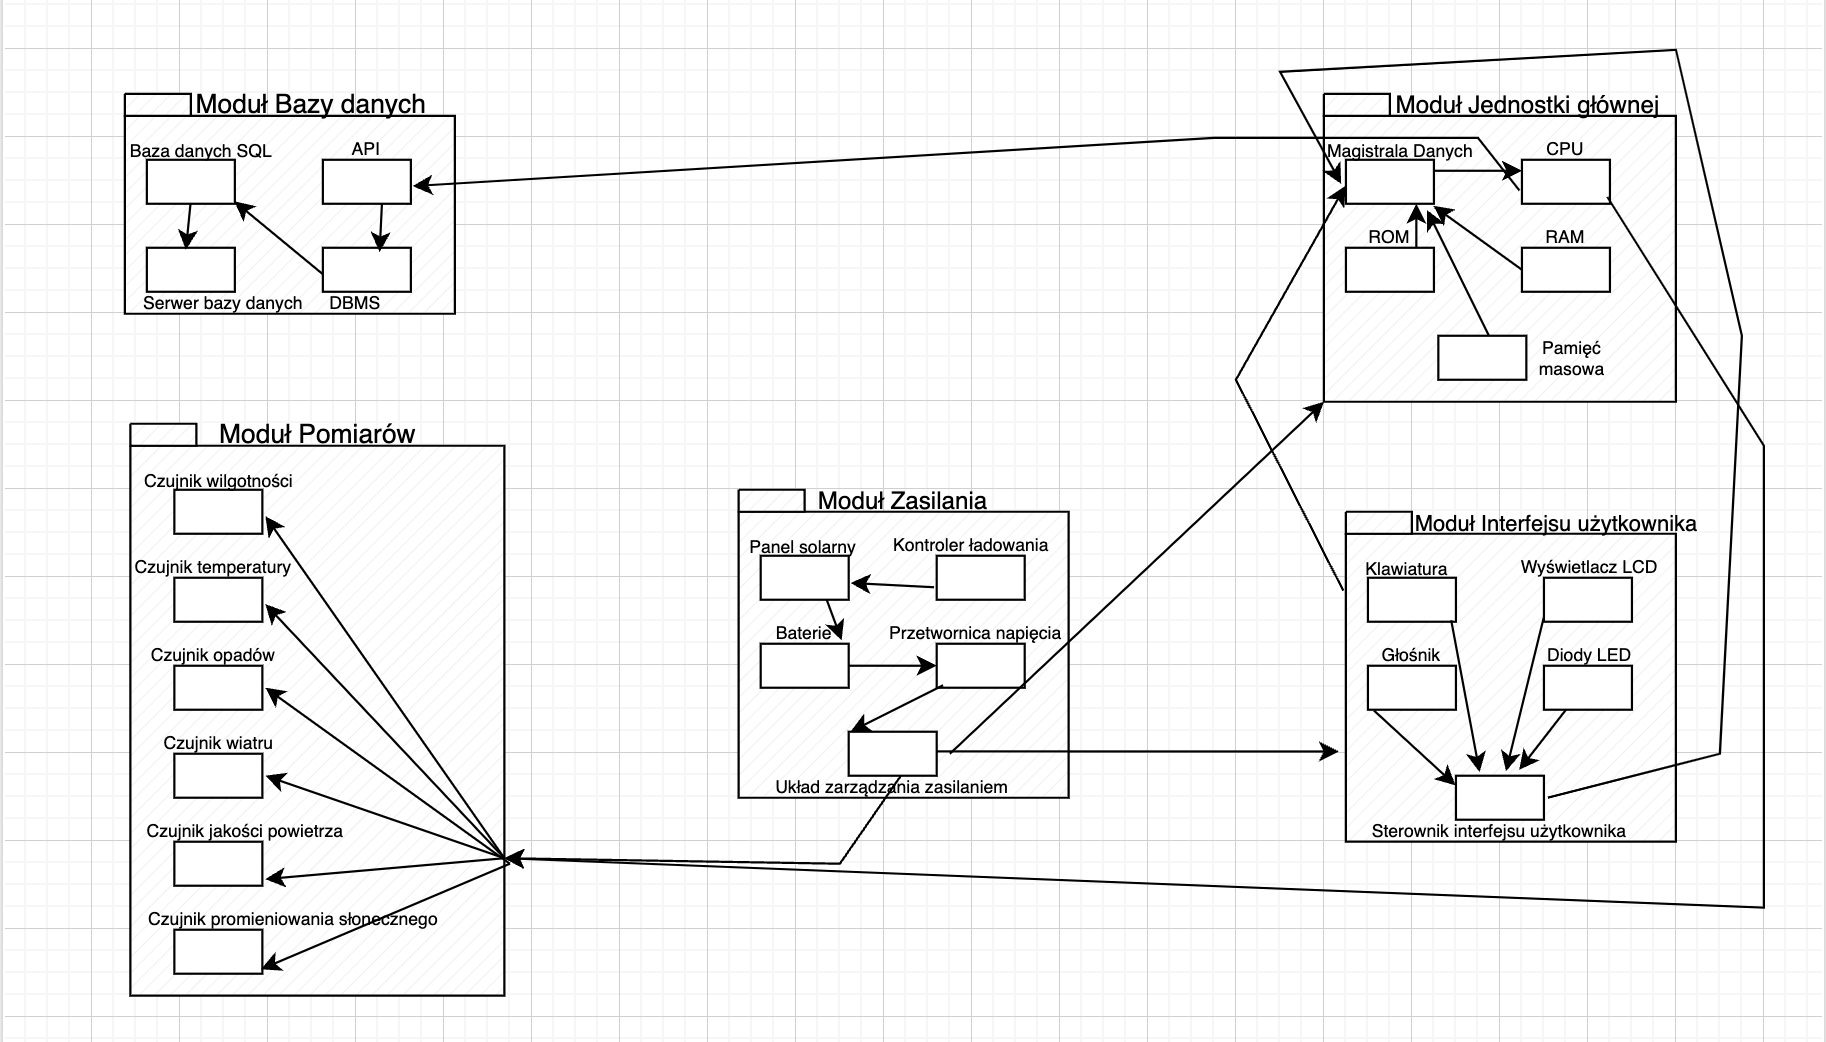
\includegraphics[scale=0.5]{moduły.png}
    \caption{Schemat modułów}
    \label{etykieta}
\end{figure}

\begin{figure}
    \centering
    \begin{minipage}{0.6\textwidth}
        \centering
        \large Pierwszy z diagramów stanów prezentuję stan "Gotowość", który opisuje sytuację inicjalizacji pracy stacji pogodowej.
    \end{minipage}
    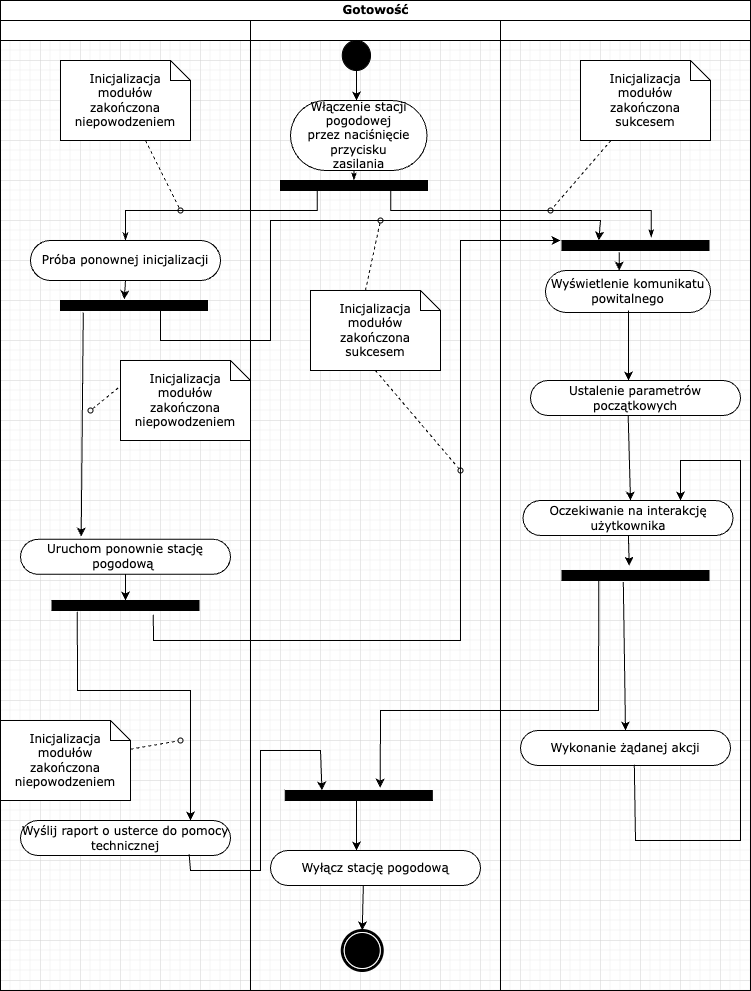
\includegraphics[scale=0.5]{gotowosc.png}
    \caption{Diagram stanu "Gotowość"}
    \label{etykieta1}
\end{figure}

\begin{figure}
    \centering
    \begin{minipage}{0.6\textwidth}
        \centering
        \large Drugi z diagramów stanów prezentuję stan "Oczekiwanie", który prezentuje działanie systemu w konteksćie odbierania sygnałów zewnętrznych i wewenętrznych związanych z podstawowym sterowaniem.
    \end{minipage}
    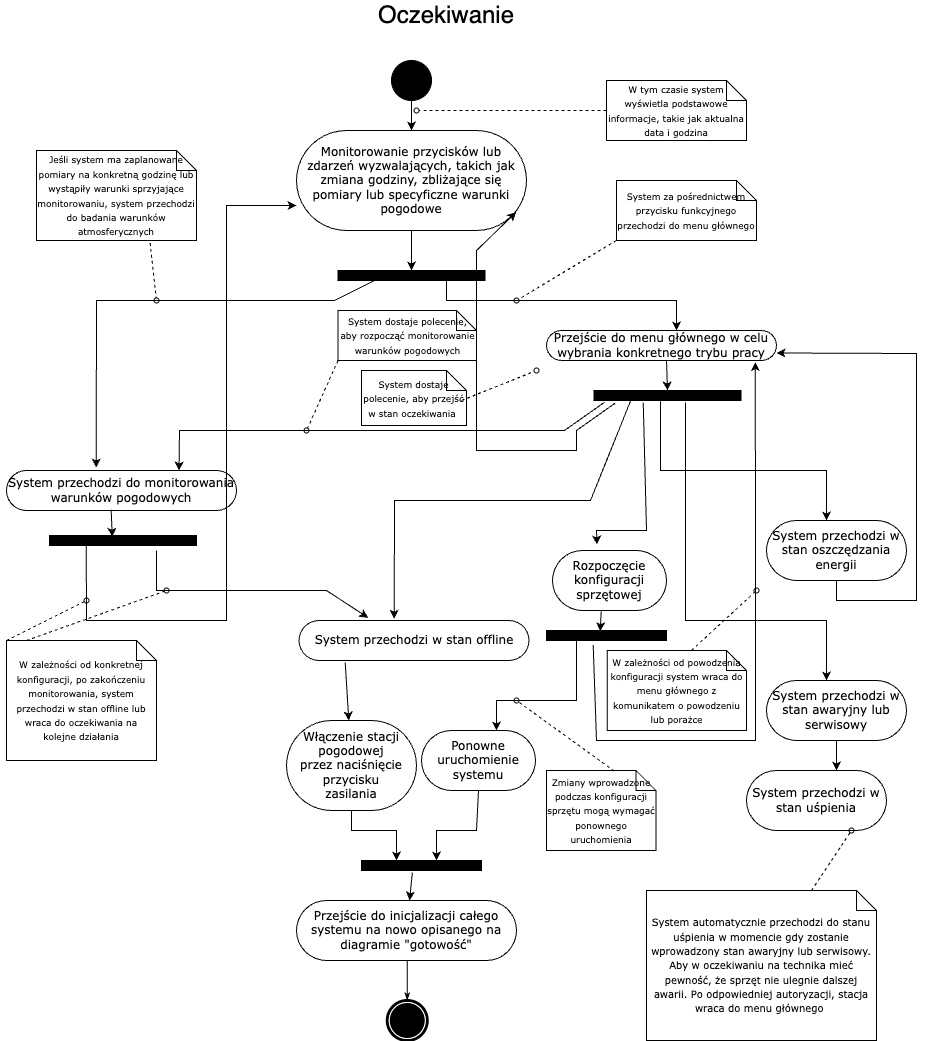
\includegraphics[scale=0.5]{oczekiwanie.png}
    \caption{Diagram stanu "Oczekiwanie"}
    \label{etykieta2}
\end{figure}
\end{document}